\documentclass[]{article}

\usepackage{amsmath, amssymb, lmodern, hyperref, parskip, xcolor, caption}

%%% Set some length and section count
\setlength{\emergencystretch}{3em}
\providecommand{\tightlist}{\setlength{\itemsep}{0pt}\setlength{\parskip}{0pt}}
\setcounter{secnumdepth}{-\maxdimen}
\captionsetup{width=0.8\linewidth, justification=centering}

%%% Set the reply style
\usepackage{tcolorbox}
\tcbuselibrary{breakable, most}
\newenvironment{reply}{\begin{quote}\vspace{0.05cm}\parskip=0.2cm}{\end{quote}}
\tcolorboxenvironment{reply}{
  blanker,
  breakable,
  before skip = 6pt,
  after skip = 12pt,
  left = 0cm,
  right = -0.5cm,
  borderline west = {2mm}{0pt}{red}
}

%%% Generate Random Words
\usepackage{lipsum}

%%% Document start
\begin{document}

\section{Reviewer(s)\textquotesingle{} Comments to Author}

\subsection{Reviewer 1}

I have a question.

\begin{reply}
No, you don't.
\end{reply}

I have another question.

\begin{reply}
No, you don't. \footnote{No, you don't.}

\begin{center}
  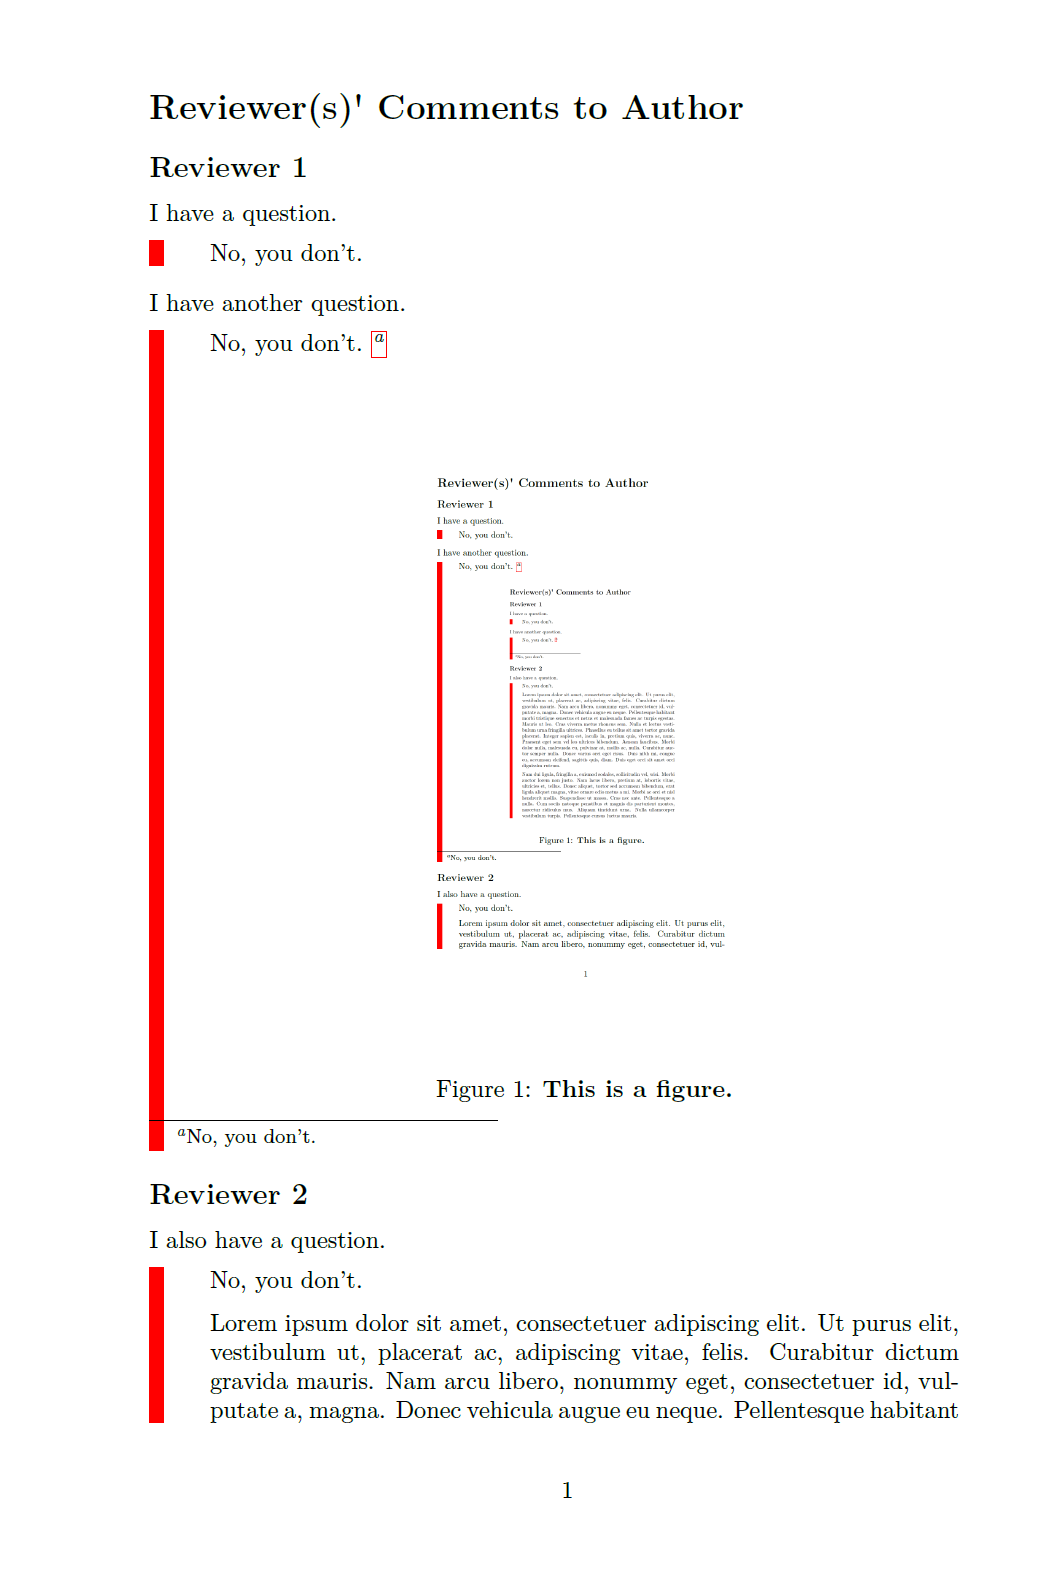
\includegraphics[width=0.5\textwidth]{figure.png}
  \captionof{figure}{\bf This is a figure.}\label{fig:1}
\end{center}
\end{reply}

\subsection{Reviewer 2}

I also have a question.
\begin{reply}
No, you don't.

\lipsum[1-2]
\end{reply}

\end{document}